% Created 2020-12-07 Mon 19:43
% Intended LaTeX compiler: pdflatex
\documentclass{article}
\usepackage[utf8]{inputenc}
\usepackage[T1]{fontenc}
\usepackage{graphicx}
\usepackage{grffile}
\usepackage{longtable}
\usepackage{wrapfig}
\usepackage{rotating}
\usepackage[normalem]{ulem}
\usepackage{amsmath}
\usepackage{textcomp}
\usepackage{amssymb}
\usepackage{capt-of}
\usepackage{hyperref}
\bibliographystyle{plain}
\author{Keagan McMahon, Brigitta Munds, \\ Benjamin Brown, \& Christina Rachmadita}
\date{\textit{<2020-12-14 Mon>} December 14th, 2020}
\title{PSYCH 363 - Stroop Effect: Congruency and Response Time}
\hypersetup{
 pdfauthor={Keagan McMahon, Brigitta Munds, \\ Benjamin Brown, \& Christina Rachmadita},
 pdftitle={PSYCH 363 - Stroop Effect: Congruency and Response Time},
 pdfkeywords={},
 pdfsubject={},
 pdfcreator={Emacs 26.3 (Org mode 9.1.9)}, 
 pdflang={English}}
\begin{document}

\maketitle
\tableofcontents

This is to test your installation of the files and programs needed to make a simple report. To compile to pdf use \texttt{C-c C-e l p}.

\section{Introduction}
\label{sec:orgbdc3519}

Insert introduction text here\ldots{}


\section{Methods}
\label{sec:org22ebc97}

Insert some method text here

This loads an R library
\begin{verbatim}
library(random)
\end{verbatim}


\section{Results}
\label{sec:org49a52bf}

Insert some results text here and other content (i.e. code, etc)

Now we will see if we can some source code and a simple plot for our export.

\begin{verbatim}
x = 1:10
y = rnorm(10)
print(mean(y))
\end{verbatim}

\begin{verbatim}
0.304133655574248
\end{verbatim}

Here is some more R source code!
\begin{verbatim}
{ a=2
  b=6
  multiply <- function(a,b)
  return(a * b)
  print(paste(a, "multiplied by", b, "is", (print(multiply(a,b)))))
}

{ for(i in seq(1,10))
if(i%%2==0){ 
print(i) }
}
\end{verbatim}

Now lets try some Python source code from my loop assignment\ldots{}

\begin{verbatim}
letters = ['t', 'r', 'i', 'b', 'q', 'v', 'h', 'p']
position = ['1st', '2nd', '3rd', '4th', '5th', '6th', '7th', '8th']

for x in letters:
  print(x)

for i in sorted(letters):
  print(i)

for x in enumerate(zip(letters, position)):
  print("The {0} letter in list 1 is {0}".format(x))

\end{verbatim}


Here is a graph of our results for you to see: 

\begin{verbatim}
plot(x,y,type = 'b')
\end{verbatim}

\begin{center}
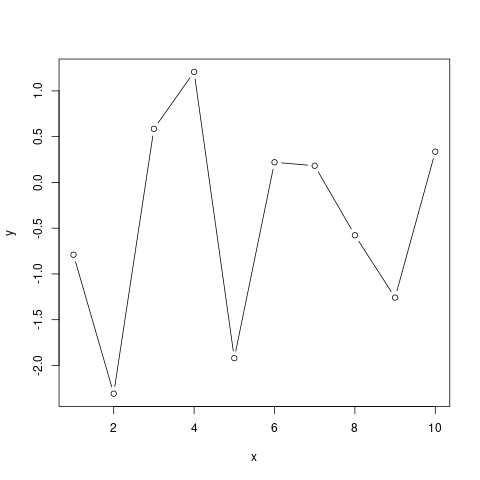
\includegraphics[width=.9\linewidth]{simplePlot.png}
\end{center}


Here is some code that produces a table of data for us:
\begin{verbatim}
d <- data.frame(foo=c('a','b','n'), bar=c(1.0/3.0,22,32))

d

\end{verbatim}

\begin{center}
\begin{tabular}{lr}
foo & bar\\
\hline
a & 0.333333333333333\\
b & 22\\
n & 32\\
\end{tabular}
\end{center}



Here is an example of an inline piece of code, it will generate 20 random numbers:
\begin{verbatim}

xinline = rnorm(20)

\end{verbatim}

We can use that code in this way:

The mean of 20 mean 0 normally distributed numbers is 0.2677680022121.


\section{Conclusions}
\label{sec:orgf5fac26}

Put some type of conlusion content here\ldots{}.



\section{References}
\label{sec:orgcdf8542}

Insert some references here, such as\ldots{}

This article \cite{britt}

\bibliography{stroopBib.bib}


\section{Testing Plots here\ldots{}..}
\label{sec:org2382b36}
\begin{verbatim}
library(ggplot2)

data <- read.csv("/home/keagan/GitRepos/363Stroop/363Stroop_Data_Dec_4.csv")

incongruent <- data[which(data$Congruent == 0),]$Time
congruent <- data[which(data$Congruent == 1),]$Time
df <- data.frame(cond = c("Incongruent", "Congruent"), rt = c(mean(incongruent), mean(congruent)))

p <- ggplot(df, aes(x = cond, y = rt, fill = cond)) + geom_bar(stat = "identity", width = 0.5) + labs(title = "Condition on Reaction Time", x = "Condition", y = "Reaction Time (s)") + theme(legend.position = "right") + theme_minimal()

p
\end{verbatim}

\begin{center}
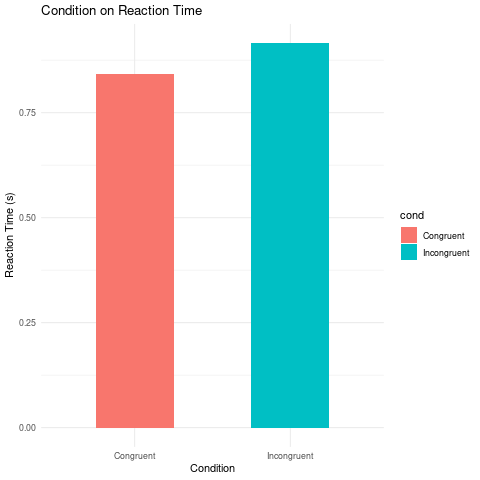
\includegraphics[width=.9\linewidth]{barplot_stroop.png}
\end{center}


\begin{verbatim}
library(ggplot2)

data <- read.csv("/home/keagan/GitRepos/363Stroop/363Stroop_Data_Dec_4.csv")

Lincongruent <- c()
counter = 1
while(counter <= 20) {
  T = data[which(data$Trial == counter & data$Congruent == 0),]
  mean_RT = mean(T$Time)
  Lincongruent = append(Lincongruent, mean_RT)
  counter = counter + 1
}

Lcongruent <- c()
counter = 1
while(counter <= 20) {
  T = data[which(data$Trial == counter & data$Congruent == 1),]
  mean_RT = mean(T$Time)
  Lcongruent = append(Lcongruent, mean_RT)
  counter = counter + 1
}

cond_rt_df <- data.frame(Condition = rep(c("Congruent", "Incongruent"), each = 20), RT = c(Lcongruent, Lincongruent))
df <- data.frame(Congruent = Lcongruent, Incongruent = Lincongruent)
df$Interference <- df$Incongruent - df$Congruent

incongruent_mean <- mean(data[which(data$Congruent == 0),]$Time)
congruent_mean <- mean(data[which(data$Congruent == 1),]$Time)
overall <- data.frame(cond = c("Incongruent", "Congruent"), rt = c(incongruent_mean, congruent_mean))

\end{verbatim}

\begin{center}

\includegraphics[width=.9\linewidth]{converted_stroop1.png}
\end{center}





\begin{verbatim}

p <- ggplot(overall, aes(x = cond, y = rt, fill = cond)) + geom_bar(stat = "identity", width = 0.5) + labs(title = "Mean Reaction Time", x = "Condition", y = "Reaction Time (s)") + theme_classic() + theme(plot.title = element_text(hjust = 0.5, size = 15, face = "bold"), legend.position = "right", legend.background = element_blank(), legend.box.background = element_rect(colour = "black"), panel.background = element_blank(), panel.grid = element_blank(), panel.border = element_rect(colour = "black", fill = NA, size = 0.75))

p

\end{verbatim}

\begin{center}

\includegraphics[width=.9\linewidth]{converted_stroop2.png}
\end{center}



\begin{verbatim}

density_plot <- ggplot(cond_rt_df, aes(x = RT, color = Condition, fill = Condition)) + geom_density(alpha = 0.5) + labs(title = "Response Time Density Plot", x = "Response Time (s)", y = "Frequency") + theme_classic() + theme(plot.title = element_text(hjust = 0.5, size = 15, face = "bold"), legend.position = "right", legend.background = element_blank(), legend.box.background = element_rect(colour = "black"), panel.background = element_blank(), panel.grid = element_blank(), panel.border = element_rect(colour = "black", fill = NA, size = 0.75)) + xlim(0.25, 1.75)

density_plot

\end{verbatim}

\begin{center}

\includegraphics[width=.9\linewidth]{converted_stroop3.png}
\end{center}



\begin{verbatim}

interference_hist <- ggplot(df, aes(x = Interference)) + geom_histogram(binwidth = 0.05, color = "white", fill = "darkturquoise") + labs(title = "Interference Histogram", x = "Increase in Response Time (s)", y = "Number of Observers") + theme_classic() + theme(plot.title = element_text(hjust = 0.5, size = 15, face = "bold"), panel.background = element_blank(), panel.grid = element_blank(), panel.border = element_rect(colour = "black", fill = NA, size = 0.75))

interference_hist

\end{verbatim}

\begin{center}

\includegraphics[width=.9\linewidth]{converted_stroop4.png}
\end{center}




\begin{verbatim}

RT_congruent <- ggplot(df, aes(x = Congruent)) + geom_histogram(alpha = 0.5, fill = "steelblue") + geom_density(color = "steelblue") + labs(title = "Response Time for Congruent Words", x = "Response Time (s)", y = "Frequency") + theme_classic() + theme(plot.title = element_text(hjust = 0.5, size = 15, face = "bold"), panel.background = element_blank(), panel.grid = element_blank(), panel.border = element_rect(colour = "black", fill = NA, size = 0.75)) + xlim(0.25, 1.75) + ylim(0, 5)

RT_congruent

\end{verbatim}

\begin{center}
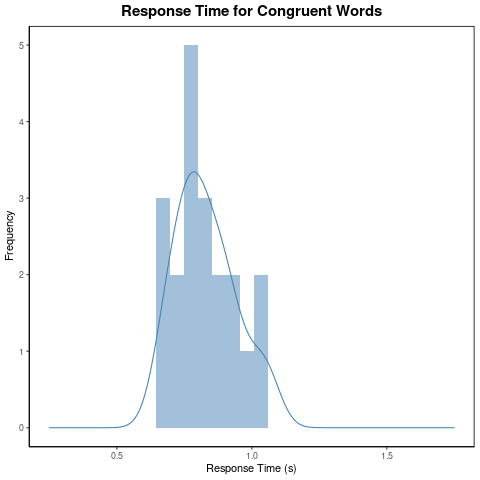
\includegraphics[width=.9\linewidth]{converted_stroop5.png}
\end{center}




\begin{verbatim}

RT_incongruent <- ggplot(df, aes(x = Incongruent)) + geom_histogram(alpha = 0.5, fill = "steelblue") + geom_density(color = "steelblue") + labs(title = "Response Time for Incongruent Words", x = "Response Time (s)", y = "Frequency") + theme_classic() + theme(plot.title = element_text(hjust = 0.5, size = 15, face = "bold"), panel.background = element_blank(), panel.grid = element_blank(), panel.border = element_rect(colour = "black", fill = NA, size = 0.75)) + xlim(0.25, 1.75) + ylim(0, 5)

RT_incongruent

\end{verbatim}

\begin{center}
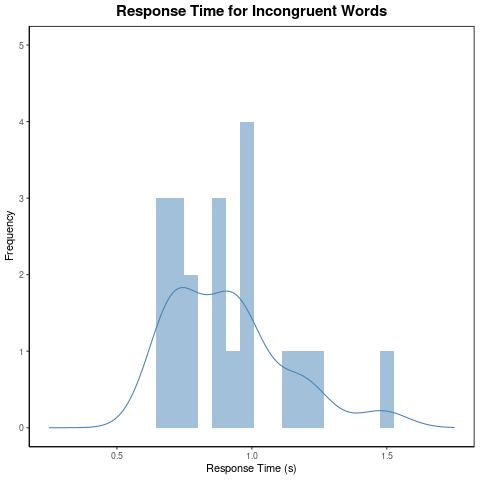
\includegraphics[width=.9\linewidth]{converted_stroop6.png}
\end{center}



\begin{verbatim}

RT_cond <- ggplot(cond_rt_df, aes(x = RT, color = Condition, fill = Condition)) + geom_histogram(color = NA, alpha = 0.5, position = "identity") + geom_density(alpha = 0) + labs(title = "Response Time for Congruent vs. Incongruent Words", x = "Response Time (s)", y = "Frequency") + theme_classic() + theme(plot.title = element_text(hjust = 0.5, size = 15, face = "bold"), legend.position = "right", legend.background = element_blank(), legend.box.background = element_rect(colour = "black"), panel.background = element_blank(), panel.grid = element_blank(), panel.border = element_rect(colour = "black", fill = NA, size = 0.75)) + xlim(0.25, 1.75) + ylim(0, 5)

RT_cond

\end{verbatim}

\begin{center}

\includegraphics[width=.9\linewidth]{converted_stroop7.png}
\end{center}
\end{document}
